
\chapter{Scenarios}

To allow researchers to evaluate learning agents in conditions of different characteristics, we provide a mechanism of scenarios.

In this chapter we define what a scenario is (see Section \ref{sec:scenario_definition}), describe sample scenarios included with the API (see Section \ref{sec:scenarios}) and point out essentials of creating custom scenarios (see Section \ref{sec:creating_scenarios}).

\section{Definition}\label{sec:scenario_definition}
Scenarios are DOOM resource files in special iwad format. A single scenario defines a map (structure of the world e.g. walls, corridors, monsters) and~a~script which determines behavior of entities and events. The script is also the place to assign rewards for various events. A scenario can define multiple maps in one iwad and~they all can be accessed by the framework. Default name for a map is `map01' but in general it can be completely arbitrary. Each map requires a separate script file.
\\
Scenarios cannot affect:
\begin{itemize}
	\item constraints regarding buttons that can and cannot be used,
	\item episode timeout,
	\item skill level (they can affect; however, everything that depands on it),
	\item any rendering options e.g. screen resolution or~crosshair visibility,
	\item framework reaction to player's death.
\end{itemize}

Due to scenarios' ability to set rewards they could be used to implement so called \emph{living~reward} and a~penalty for dying. Nonetheless, using API's \emph{setLivingReward} and \emph{setDeathPenalty} methods (see //REFERENCE HERE//).

\section{Tools}\label{sec:tools}
\begin{figure}
		\centering
		\includegraphics[scale=0.3]{slade.png}
		\caption{Slade 3 application for scenario creation.}\label{fig:slade}
	\end{figure}

Creating iwad files involves compilation thus~requires a dedicated software. \emph{Slade~3} and \emph{Doom~Builder~2}  were our editors of choice because of huge popularity, availability of resources and~relative quality. The editors differ mostly in user interface details but~both provide most curcial functionalities:

\begin{itemize}
	\item \textbf{visual map editor} - a simple tool for map creation which is very easy to use and~enables you to achieve whatever is possible in Doom engine.
	\item \textbf{Action Code Script support} - dedicated language resembling C that is suitable for determining behavior of any monster, player and~object in the game.
	\item \textbf{testrunning} - possibility to test your scenario without resorting to external software or~calls. Test running requires providing a \emph{zdoom} executive file and \emph{doom2.wad} file (or~any other basic resource file) . 
\end{itemize}

Both tools are robust, reasonably easy to use and~provide much elasticity in sceanrio creation. However, due to the lack of native \emph{Linux} support and~some bad design solutions (mainly concerning interface) we consider \emph{Doom~Builder~2} a slightly inferior choice. 

\newpage
\section{Provided Scenarios}\label{sec:scenarios}
\subsection{Basic}\label{subsec:basic}
	
	\begin{figure}
		\centering
		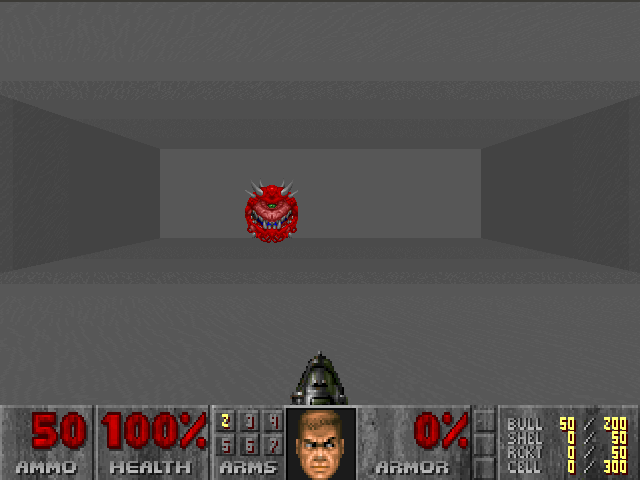
\includegraphics[scale=0.5]{basic.png}
		\caption{Doom gameplay frame from `basic' scenario.}\label{fig:basic}
	\end{figure}
\begin{itemize}
	\item motivation 
	\item description
\end{itemize}

\newpage
\subsection{Deadly Corridor}
	\begin{figure}
		\centering
		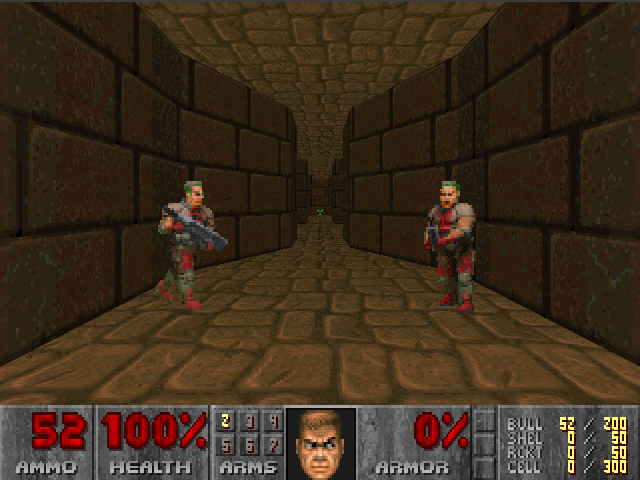
\includegraphics[scale=0.5]{deadly_corridor.png}
		\caption{Doom gameplay frame from `deadly corridor' scenario.}\label{fig:deadly_corridor}
	\end{figure}
\begin{itemize}
	\item motivation
	\item description
\end{itemize}
\newpage

\subsection{Defend the Center}
	\begin{figure}
		\centering
		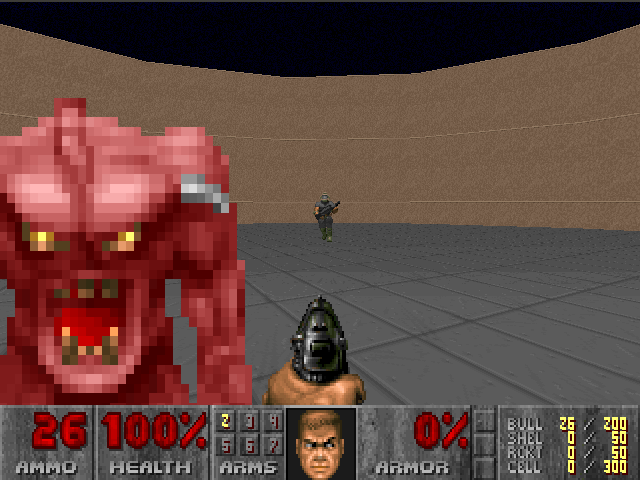
\includegraphics[scale=0.5]{defend_the_center.png}
		\caption{Doom gameplay frame from `defend the center' scenario.}\label{fig:basic}
	\end{figure}
\begin{itemize}
	\item motivation
	\item description
\end{itemize}

\newpage
\subsection{Defend the Line}
	\begin{figure}
		\centering
		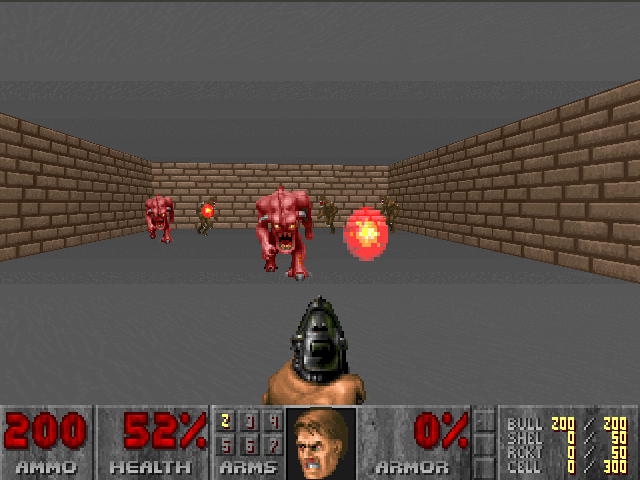
\includegraphics[scale=0.5]{defend_the_line.png}
		\caption{Doom gameplay frame from `defend the line' scenario.}\label{fig:defend_the_line}
	\end{figure}
\begin{itemize}
	\item motivation
	\item description
\end{itemize}

\newpage
\subsection{Deathmatch}
	\begin{figure}
		\centering
		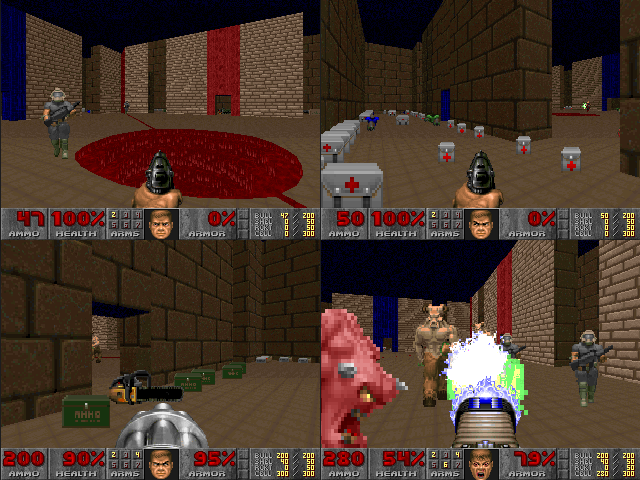
\includegraphics[scale=0.5]{deathmatch.png}
		\caption{4 Doom gameplay frames from `deathmatch' scenario.}\label{fig:deatchmatch}
	\end{figure}
\begin{itemize}
	\item motivation
	\item description
\end{itemize}


\newpage
\subsection{Health Gathering}
	\begin{figure}
		\centering
		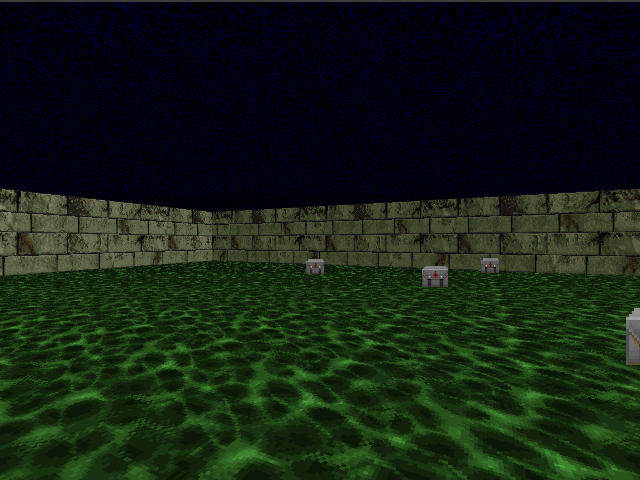
\includegraphics[scale=0.5]{health_gathering.png}
		\caption{Doom gameplay frame from `health gathering' scenario.}\label{fig:health_gathering}
	\end{figure}
\begin{itemize}
	\item motivation
	\item description
\end{itemize}

\newpage
\subsection{My Way Home}
	\begin{figure}
		\centering
		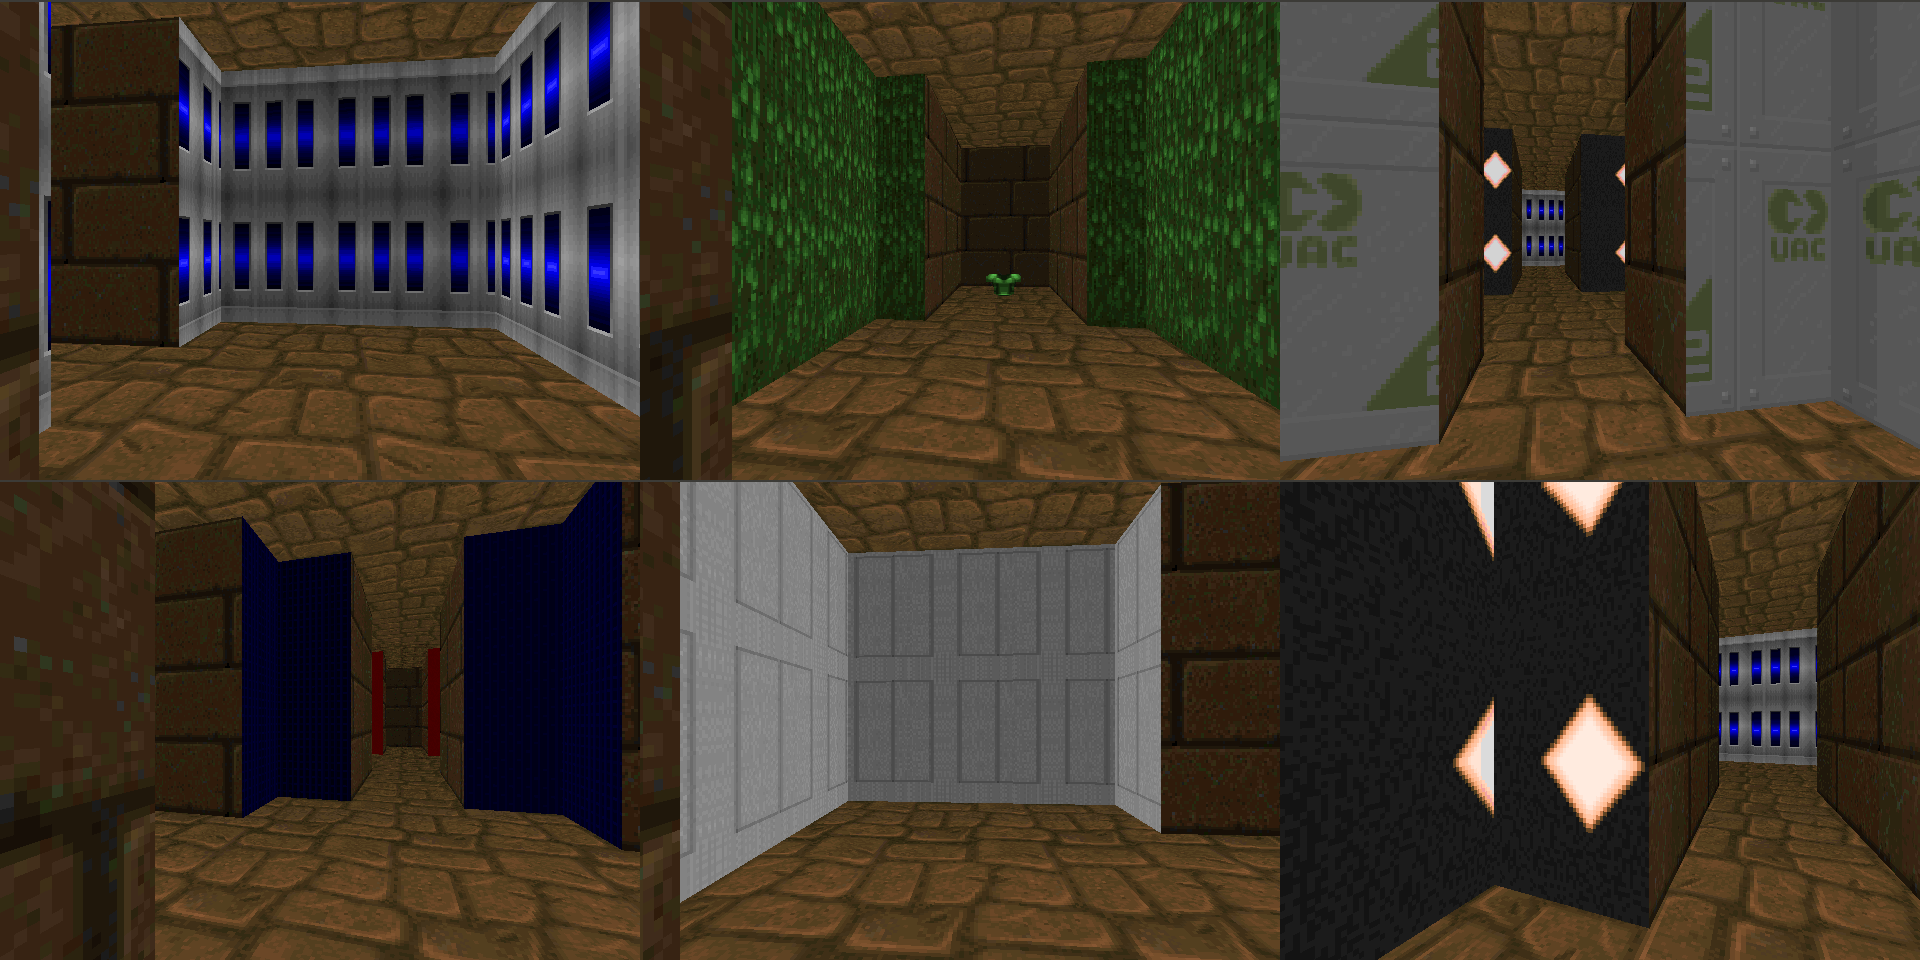
\includegraphics[scale=0.22]{my_way_home.png}
		\caption{6 Doom gameplay frames from `my way home' scenario.}\label{fig:my_way_home}
	\end{figure}
\begin{itemize}
	\item motivation
	\item description
\end{itemize}

\newpage
\subsection{Predict Position}
	\begin{figure}
		\centering
		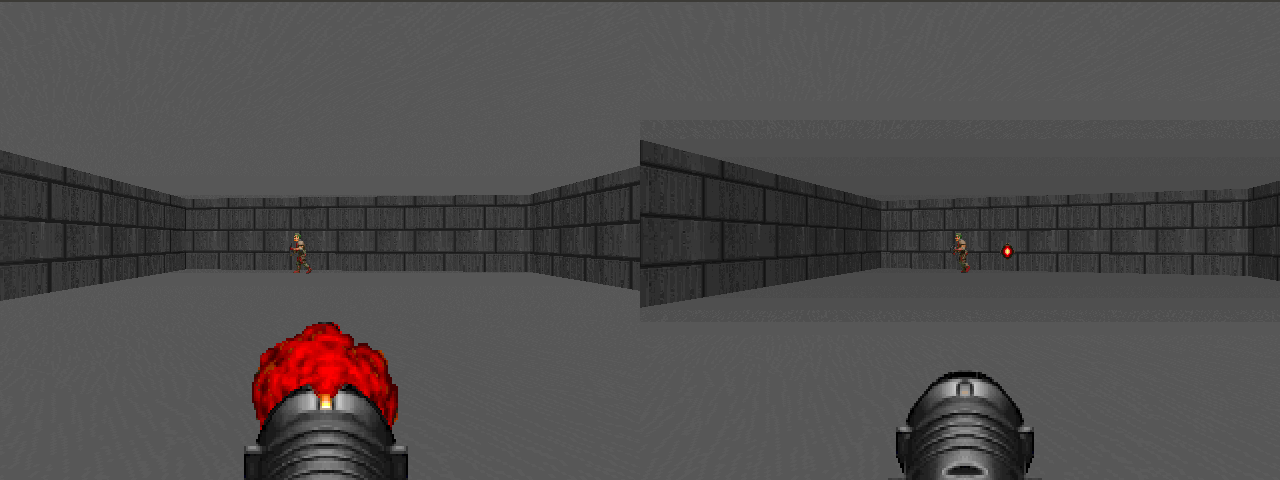
\includegraphics[scale=0.32]{predict_position.png}
		\caption{2 Doom gameplay frames from `predict position' scenario.}\label{fig:predict_position}
	\end{figure}
\begin{itemize}
	\item motivation
	\item description
\end{itemize}

\newpage
\subsection{Take Cover}
	\begin{figure}
		\centering
		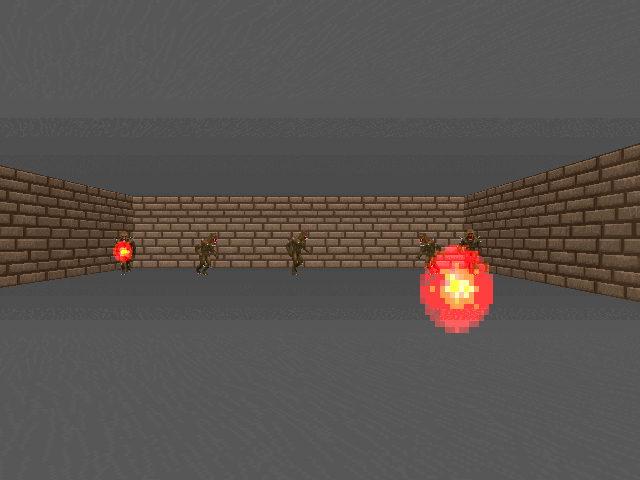
\includegraphics[scale=0.5]{take_cover.png}
		\caption{Doom gameplay frame from `take cover' scenario.}
	\end{figure}
\begin{itemize}
	\item motivation
	\item description
\end{itemize}



\section{Creating scenarios}\label{sec:creating_scenarios}
\subsection{Reward}
\subsection{User Variables}
How to easily achieve some most common tasks in acs scripts which are not so obvious and~were used here.
e.g. shaping rewards, infinite ammo, respawning, friendly monsters, 

\section{Resources}